\newprob{1715500951}
{
    把一個質量 0.5 kg 的小球拋向斜坡。小球在比拋 出之處高 \qty{2}{m} 的地方撞上斜坡後反彈。假設碰撞 時沒有能量損耗。\bigskip
    {\par\centering
        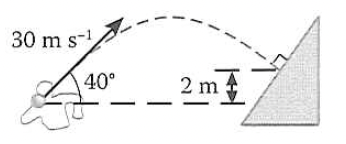
\includegraphics[width=.35\textwidth]{assets/157e649d.png}
        \par}\bigskip
    求小球彈回原位時的速率。
    \begin{tasks}
        \task \vel{10}
        \task \vel{20}
        \task \vel{23}
        \task \vel{30}
    \end{tasks}
}{D}

\newprob{1715501009}
{
    砲彈以仰角 \dg{15} 射出,落在 \qty{100}{m} 外同一高度的 地面上。若以同一初速,改為垂直朝天發射,彈 道的最高點有多高? (提示:$\sin\,2\theta=2\sin\,\theta\,\cos\,\theta$)
    \begin{tasks}
        \task \qty{100}{m}
        \task \qty{80}{m}
        \task \qty{60}{m}
        \task \qty{40}{m}
    \end{tasks}
}{D}

\newprob{1715501023}
{
    今有粒子一顆,作拋體運動,如圖。\bigskip
    {\par\centering
        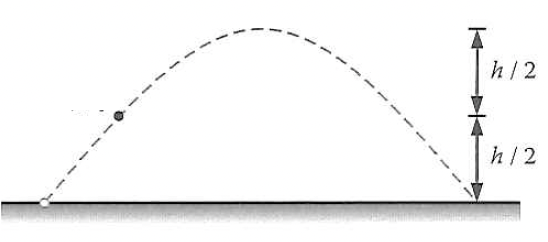
\includegraphics[width=.4\textwidth]{assets/4d5ef752.png}
        \par}
    \bigskip
    當粒子升至最高點一半的高度,
    \begin{tasks}
        \task 動能亦為初始值的一半。
        \task 垂直速率亦為初始值的一半。
        \task 所歷時間為全程的四分之一。
        \task 所增勢能為最大勢能的一半。
    \end{tasks}
}{D}

\newprob{1715501056}
{
    從同一位置,以同一速率,把兩顆粒子以不同仰 角射出。仰角一高一低,高者 \dg{50} ,低者 \dg{40} 。略 去空氣阻力不計。兩者跌回同一高度時,
    \begin{statements}
        \task 位置相同。
        \task 時間相同。
        \task 速率相同。
    \end{statements}
    \begin{tasks}
        \task 只有(2)
        \task 只有(3)
        \task 只有(1)和(2)
        \task 只有(1)和(3)
    \end{tasks}
}{D}

\newprob{1715501142}
{
    把彈丸從地面以初速 \vel{10} 仰角 \dg{30} 發射。 彈丸曲墜到遠處的桌子上。桌面離地 \qty{1}{m} 。\bigskip
    {\par\centering
        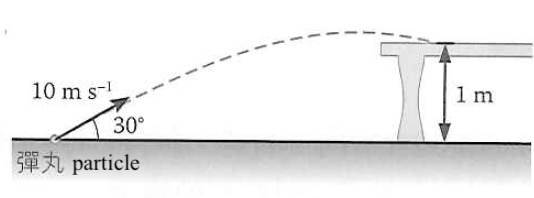
\includegraphics[width=.4\textwidth]{assets/0c28069a.png}
        \par}\bigskip
    彈丸飛行的時間是多少?
    \begin{tasks}
        \task \qty{1.640}{s}
        \task \qty{0.746}{s}
        \task \qty{0.273}{s}
        \task \qty{0.124}{s}
    \end{tasks}
}{B}

\newprob{1715501200}
{
    把小球以初速$u$、仰角 $\theta$ 拋起。小球升至最高點 後下墜,撞向牆壁。碰撞前的一刻,速度$v$與鉛 垂線的夾角亦為 $\theta$ 。\bigskip
    {\par\centering
        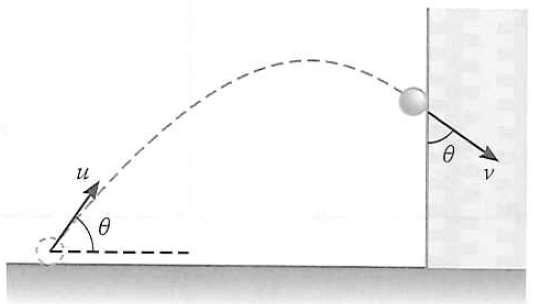
\includegraphics[width=.4\textwidth]{assets/7eb2fb07.png}
        \par}\bigskip
    從拋起至碰撞,全程歷時多久?
    \begin{tasks}
        \task $\dfrac{u}{g\sin\,\theta}$
        \task $\dfrac{u}{g\cos\,\theta}$
        \task $\dfrac{u(\cos^2\,\theta-\sin^2\,\theta)}{g\sin\,\theta}$
        \task $\dfrac{u(\sin^2\,\theta-\cos^2\,\theta)}{g\cos\,\theta}$
    \end{tasks}
}{A}

\newprob{1715501430}
{
    $P$、$Q$兩球從地面以同一初速,斜向上拋。下圖 顯示兩者的水平位移$x$隨時間的變化。\bigskip
    {
        \par
        \centering
        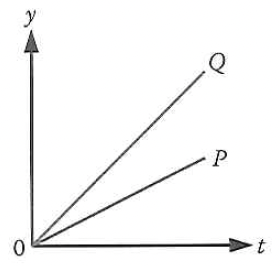
\includegraphics[width=0.3\linewidth]{assets/image.png}
        \par
    }\bigskip
    下列哪項最能顯示兩者的垂直位移$y$隨時間的變 化?
    \begin{tasks}(2)
        \task
        \topalign{
            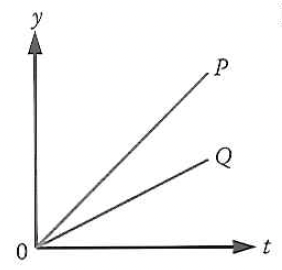
\includegraphics[width=0.55\linewidth]{assets/image1.png}
        }
        \task
        \topalign{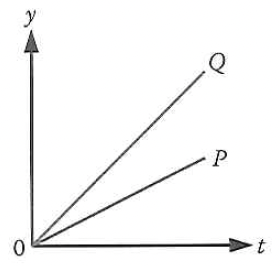
\includegraphics[width=0.55\linewidth]{assets/image.png}}
        \task
        \topalign{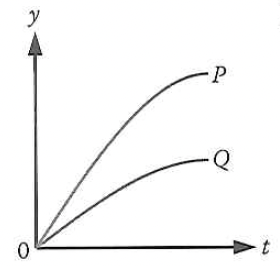
\includegraphics[width=0.55\linewidth]{assets/image2.png}}
        \task
        \topalign{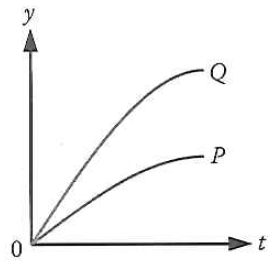
\includegraphics[width=0.55\linewidth]{assets/3.png}}
    \end{tasks}
}{D}

\newprob{1715501661}
{
    砲彈以仰角$\theta$發射,在時間$t_1$,升至最高點。下 列哪幅線圖最能顯示其動能隨時間的變化?
    \begin{tasks}(2)
        \task
        \topalign{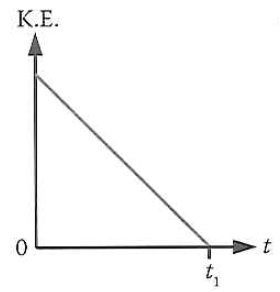
\includegraphics[width=0.55\linewidth]{assets/5.png}}

        \task
        \topalign{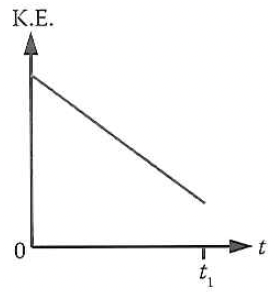
\includegraphics[width=0.55\linewidth]{assets/dwage.png}}


        \task
        \topalign{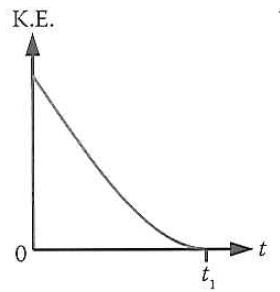
\includegraphics[width=0.55\linewidth]{assets/11.png}}


        \task
        \topalign{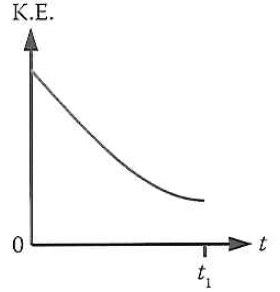
\includegraphics[width=0.55\linewidth]{assets/dqwdqwd.png}}


    \end{tasks}
}{D}

\newprob{1715501706}
{
    在高度$h$水平擲出小球,初速為$u$,如圖。小球 在時間$t_0$撞地反彈,然後在時間$t_1$去升回原來的 高度。假設地面為水平。\medskip
    {\par\centering
        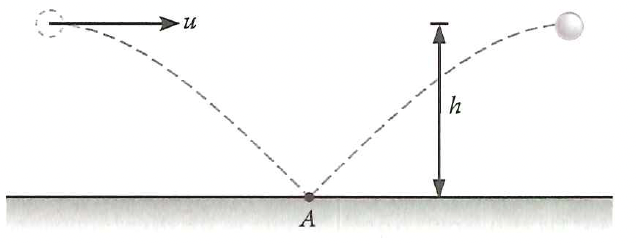
\includegraphics[width=0.5\linewidth]{assets/dqwdqd.png}\par}
    \medskip\par 下列哪幅線圖最能顯示垂直速度$v_y$,和水平速度 $v_x$。隨時間$t$的變化?
    \begin{tasks}
        \task
        \topalign{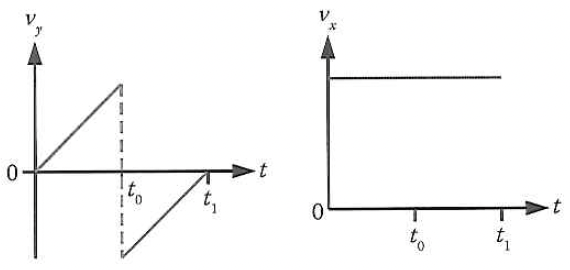
\includegraphics[width=0.5\linewidth]{assets/dwqdge.png}}


        \task
        \topalign{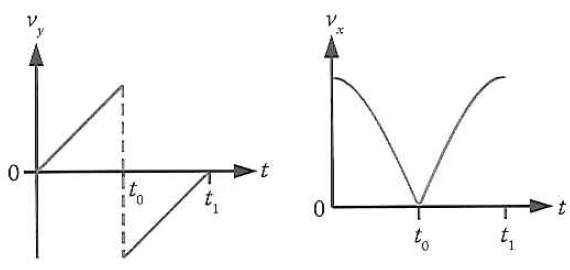
\includegraphics[width=0.5\linewidth]{assets/dmage.png}}


        \task
        \topalign{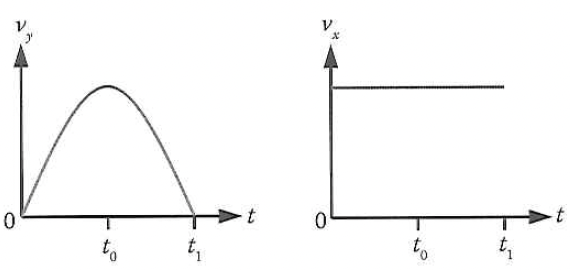
\includegraphics[width=0.5\linewidth]{assets/dqwdq.png}}


        \task
        \topalign{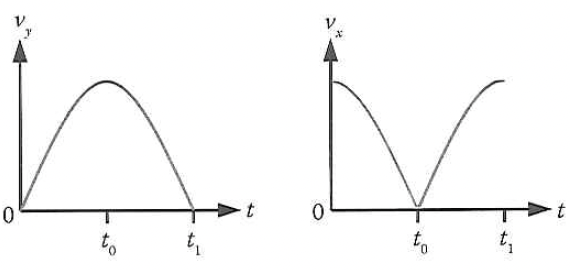
\includegraphics[width=0.5\linewidth]{assets/adasda.png}}
    \end{tasks}
}{A}

\newprob{1715501736}
{
有一條彎曲的光滑軌道,自上而下,如圖。把鋼 珠放到軌道頂端,持定,放手,讓它沿軌道滑 下。鋼珠衝出軌道 0.4 s 後着地,落點離軌道末 端的水平距離為 2 m。
{\par\centering
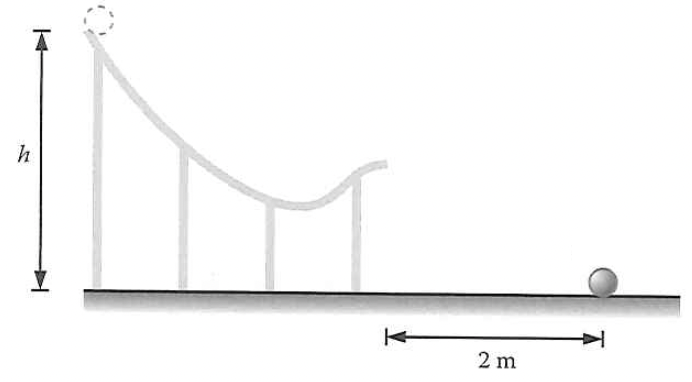
\includegraphics[width=0.45\linewidth]{assets/sasd.png}
\par
}

假設鋼珠以水平方向衝出軌道。軌道頂端的高度 $h$是多少?
\begin{tasks}
    \task \qty{0.79}{m}
    \task \qty{1.27}{m}
    \task \qty{2.06}{m}
    \task \qty{4.12}{m}
\end{tasks}
}{C}

\newprob{1715501755}
{
    水平而光滑的高台上有一件物體爆炸,裂成$A$、 $B$兩塊碎片,水平左右飛出,最後落到同一高度 的地面上。$A$、$B$ 的質量為$m$與$2m$,水平位移為$d_A$與$d_B$。
    \par{\par\centering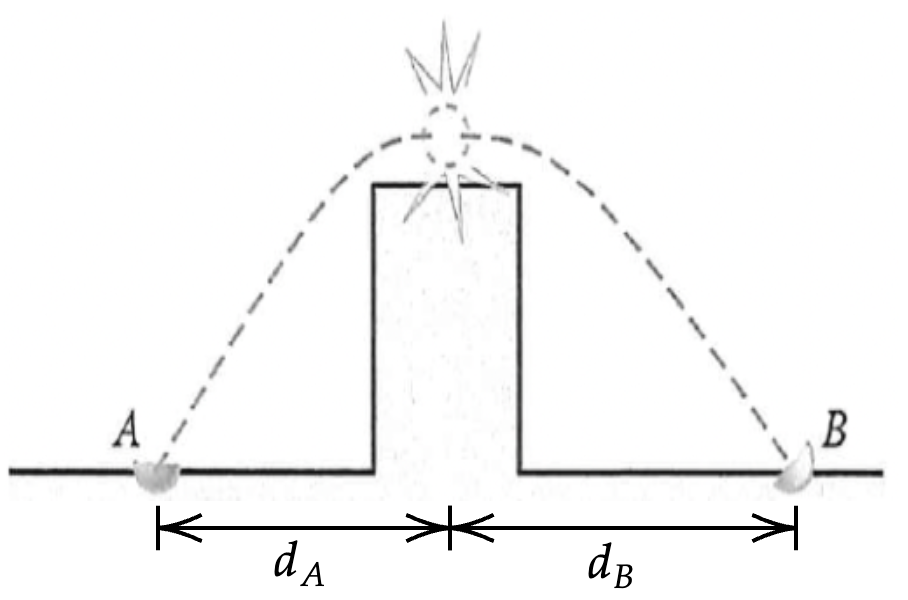
\includegraphics[width=.4\textwidth]{./img/ch6_projectile_mc_2024-05-12-16-19-49.png}\par}
    \par 兩者的水平位移之比$d_A:d_B$是多少?
    \begin{tasks}
        \task $1:1$
        \task $1:2$
        \task $2:1$
        \task $4:1$
    \end{tasks}
}{C}